\documentclass[a4paper,10pt]{article}

\usepackage[utf8]{inputenc}
\usepackage{epsfig}
\usepackage{amsmath}
\usepackage{amssymb}
\usepackage{array}
\usepackage{float} 
\usepackage{ctable}
\usepackage{multirow}
\usepackage{graphicx}
\usepackage{caption}
\usepackage{subcaption}
\usepackage{amsfonts}
\usepackage{cite}
\usepackage{algorithmic}

\title{Population Dynamics}
\author{Carlos Barreto}

\begin{document}

\maketitle


\section{Examples}
We show examples of two games that have different number of populations and strategies per population.

\subsection{Rock-paper-scissors game}
We implement the rock-paper-scissors game. This game has only one population with three strategies, denoted $x = [x_1, x_2, x_3]^\top$. The fitness function is defiined as $F(x)=Ax$, where A is equal to 
\begin{equation}
  A = \begin{pmatrix}
  0  & -1 &  1 \\
  1  &  0 & -1 \\
  -1 &  1 & 0
  \end{pmatrix}
\end{equation}


\begin{figure}
  \centering
  \begin{subfigure}[b]{0.45\textwidth}
	  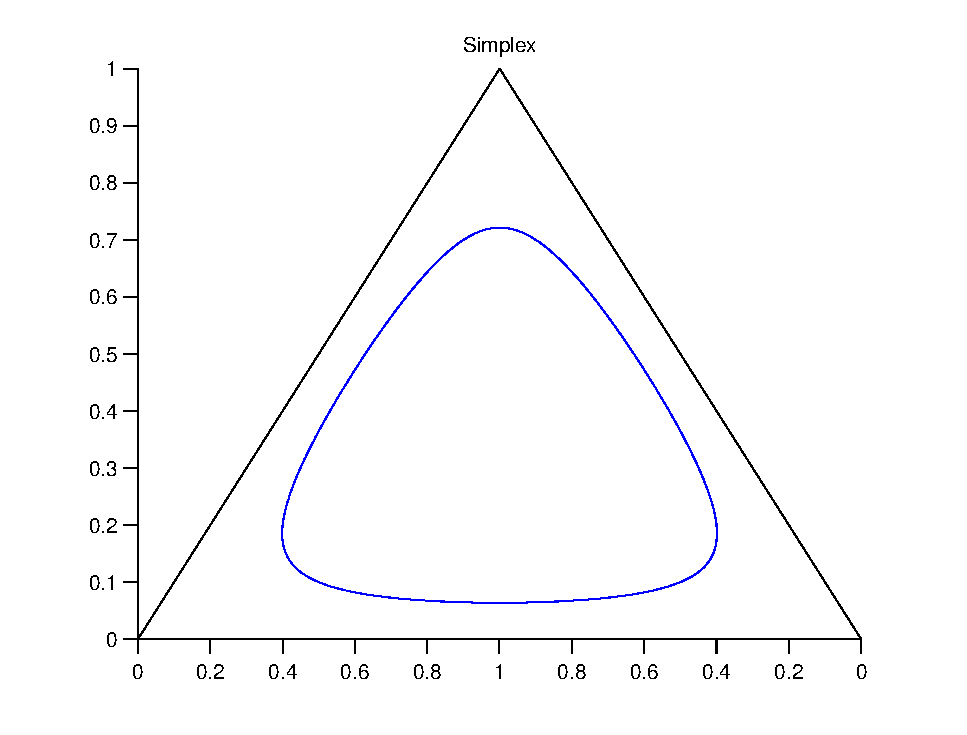
\includegraphics[width=\textwidth]{./images/test1_simplex_rd.eps}
	  \caption{Simplex.}
	  \label{fig:test1_simplex_rd}
  \end{subfigure}
  ~ 
  \begin{subfigure}[b]{0.45\textwidth}
	  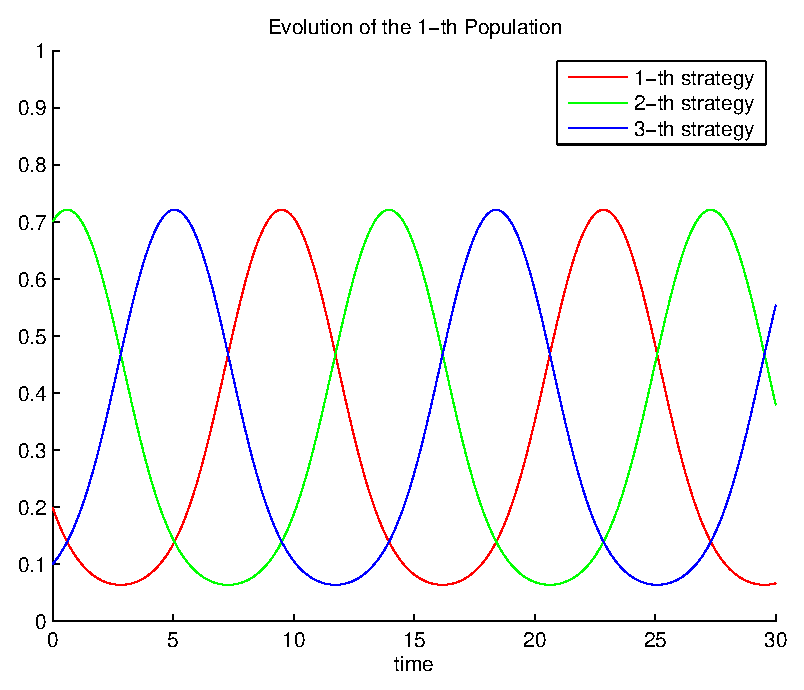
\includegraphics[width=\textwidth]{./images/test1_ev_rd.eps}
	  \caption{Evolution of the strategies in time.}
	  \label{fig:test1_ev_rd}
  \end{subfigure}
  \caption{Rock-paper-scissors game with replicator dynamics.}
  \label{fig:rpc_game_rd}
\end{figure}


\begin{figure}
  \centering
  \begin{subfigure}[b]{0.45\textwidth}
	  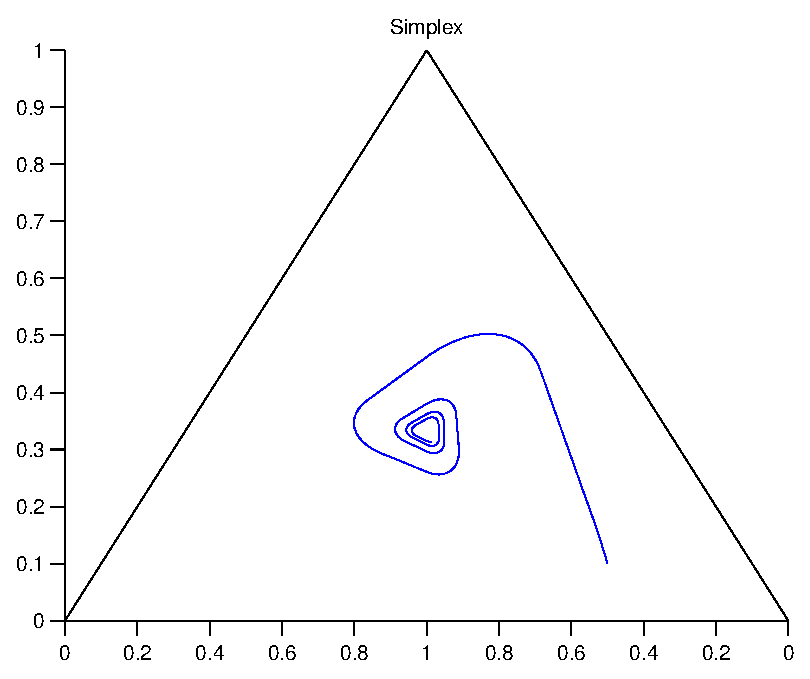
\includegraphics[width=\textwidth]{./images/test1_simplex_bnn.eps}
	  \caption{Simplex.}
	  \label{fig:test1_simplex_bnn}
  \end{subfigure}
  ~ 
  \begin{subfigure}[b]{0.45\textwidth}
	  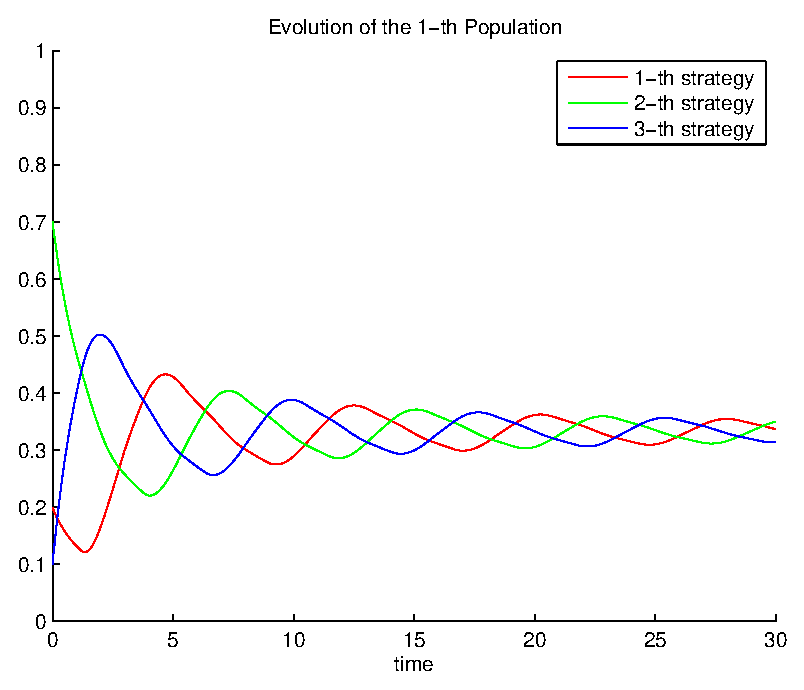
\includegraphics[width=\textwidth]{./images/test1_ev_bnn.eps}
	  \caption{Evolution of the strategies in time.}
	  \label{fig:test1_ev_bnn}
  \end{subfigure}
  \caption{Rock-paper-scissors game with BNN dynamics.}
  \label{fig:rpc_game_bnn}
\end{figure}



\begin{figure}
  \centering
  \begin{subfigure}[b]{0.45\textwidth}
	  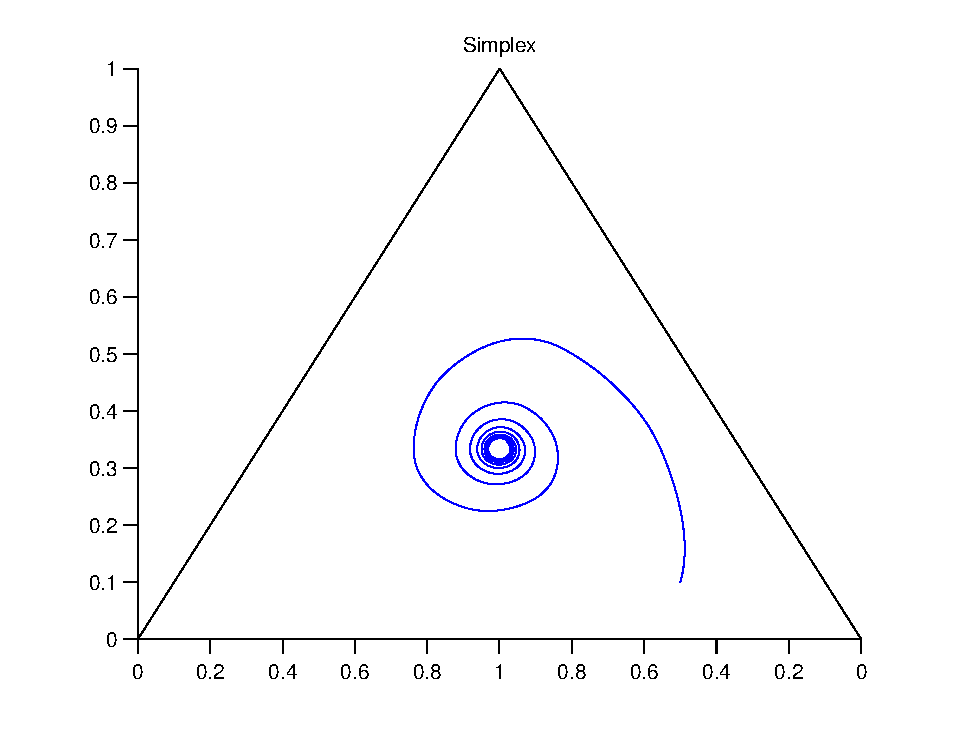
\includegraphics[width=\textwidth]{./images/test1_simplex_smith.eps}
	  \caption{Simplex.}
	  \label{fig:test1_simplex_smith}
  \end{subfigure}
  ~ 
  \begin{subfigure}[b]{0.45\textwidth}
	  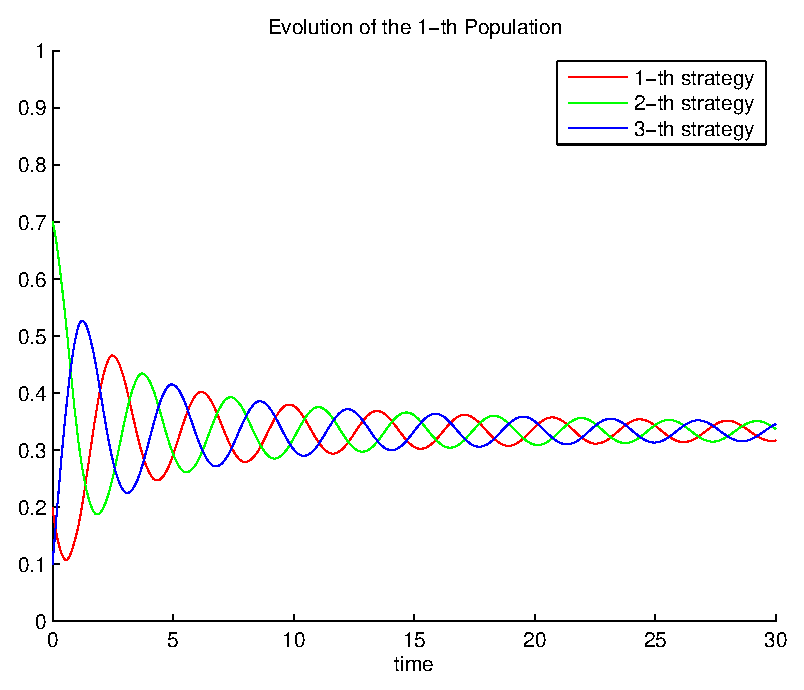
\includegraphics[width=\textwidth]{./images/test1_ev_smith.eps}
	  \caption{Evolution of the strategies in time.}
	  \label{fig:test1_ev_smith}
  \end{subfigure}
  \caption{Rock-paper-scissors game with Smith dynamics.}
  \label{fig:rpc_game_smith}
\end{figure}



\begin{figure}
  \centering
  \begin{subfigure}[b]{0.45\textwidth}
	  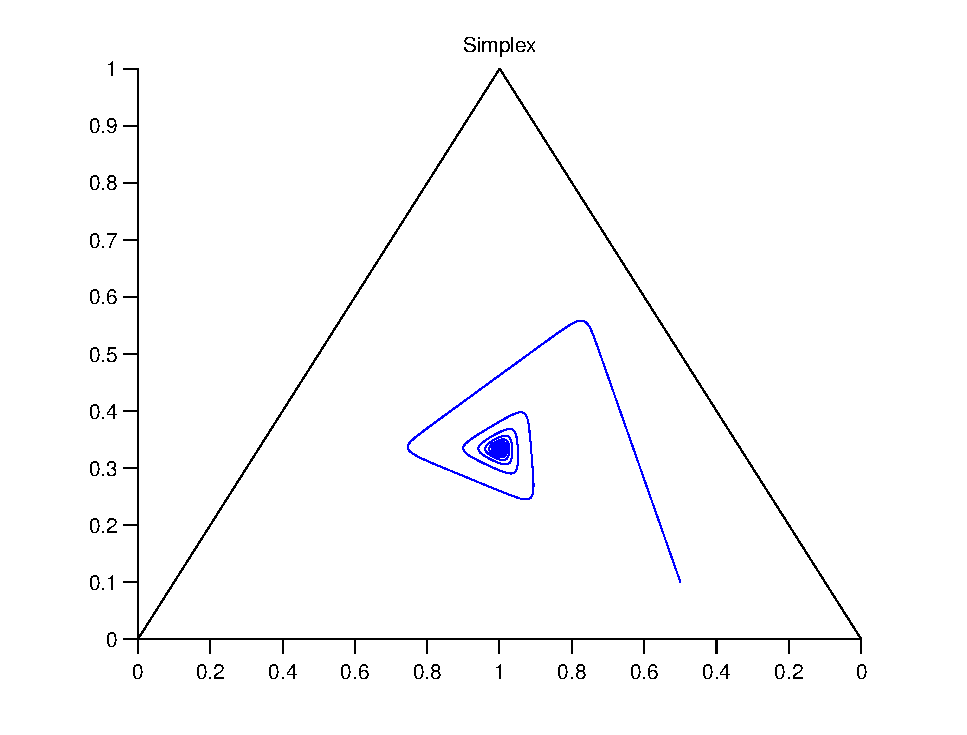
\includegraphics[width=\textwidth]{./images/test1_simplex_logit.eps}
	  \caption{Simplex.}
	  \label{fig:test1_simplex_logit}
  \end{subfigure}
  ~ 
  \begin{subfigure}[b]{0.45\textwidth}
	  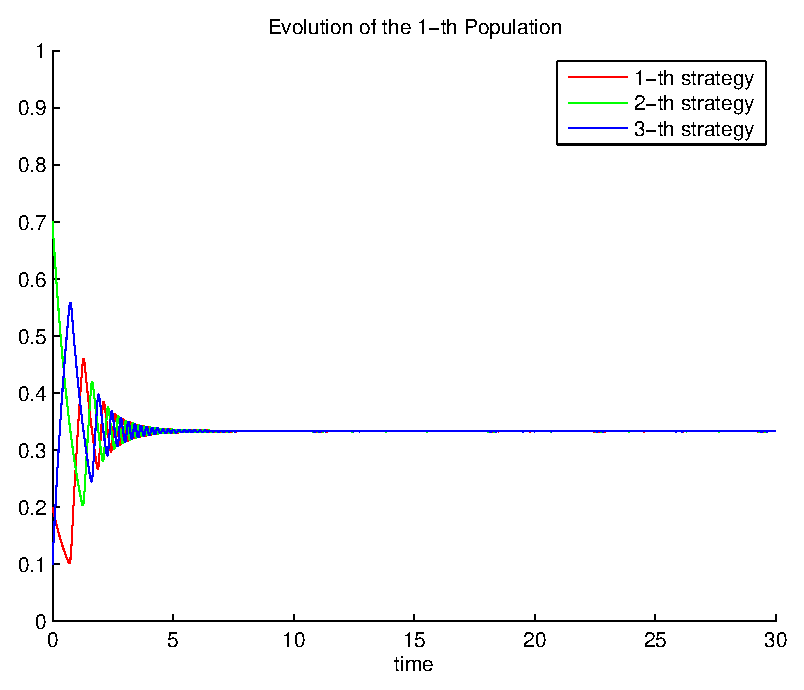
\includegraphics[width=\textwidth]{./images/test1_ev_logit.eps}
	  \caption{Evolution of the strategies in time.}
	  \label{fig:test1_ev_logit}
  \end{subfigure}
  \caption{Rock-paper-scissors game with logit dynamics.}
  \label{fig:rpc_game_logit}
\end{figure}





\subsection{Matching pennies}
We implement a matching pennies game with two populations. First, note that the payoff of the game in normal form is
%
\begin{table}[h]
\centering
 \begin{tabular}{|c|c|} \hline
  2, 1 & 1, 2 \\ \hline
  1, 2 & 2, 1 \\ \hline
 \end{tabular}
\end{table}
%
In this case each population has two strategies, namely \emph{heads} and \emph{tails}.
Now, the fitness of the $i^{th}$ population can be expressed as $F^i(x^i) = A_i x^i$, for $i=\{x_h^i, x_t^i\}$. 
The payoff matrices are defines as follows
%
\begin{equation}
  A_1 = \begin{pmatrix}
2 & 1 \\
1 & 2 
  \end{pmatrix}
\end{equation}
%
\begin{equation}
  A_2 = \begin{pmatrix}
  1 & 2 \\
  2 & 1 
  \end{pmatrix}
\end{equation}
%


\begin{figure}
  \centering
  \begin{subfigure}[b]{0.45\textwidth}
	  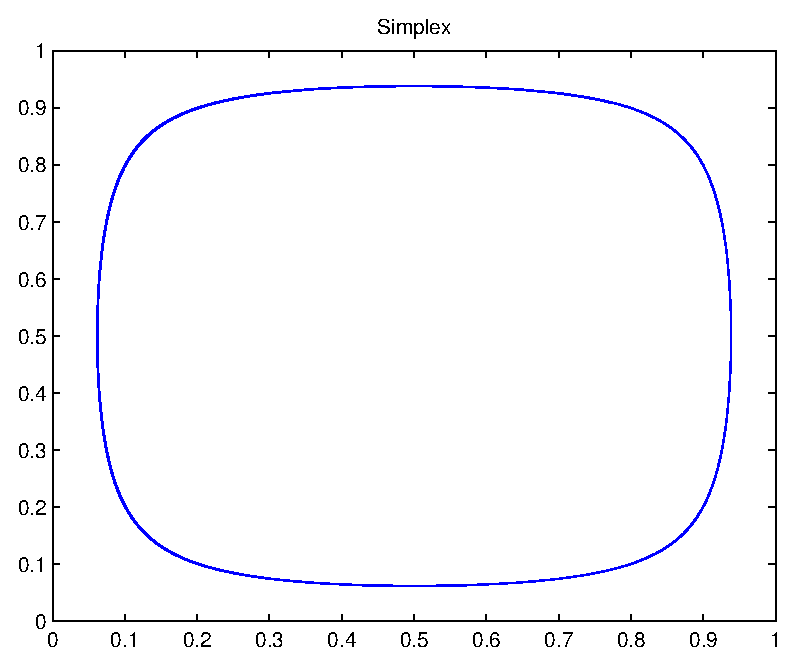
\includegraphics[width=\textwidth]{./images/test2_simplex_rd.eps}
	  \caption{Simplex.}
	  \label{fig:test2_simplex_rd}
  \end{subfigure}
  ~ 
  \begin{subfigure}[b]{0.45\textwidth}
	  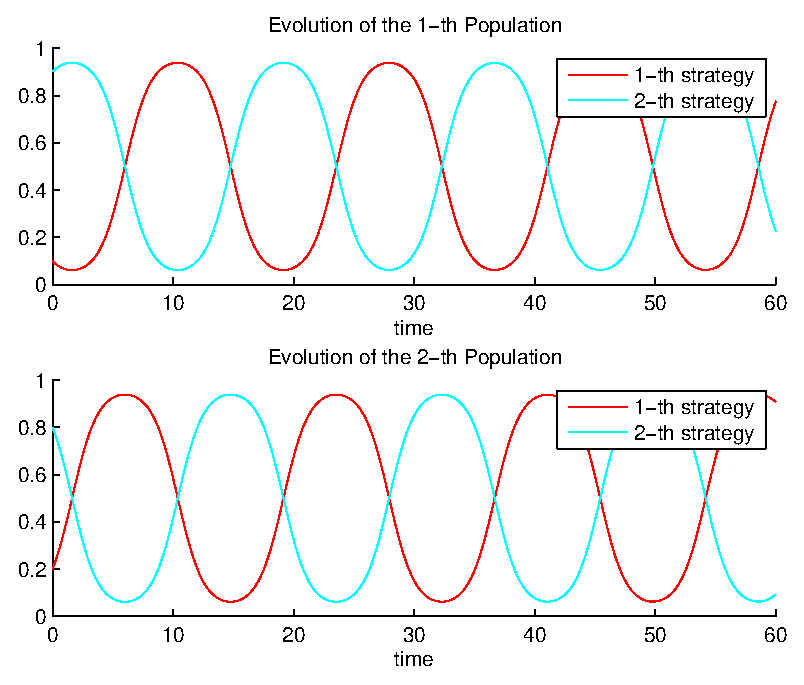
\includegraphics[width=\textwidth]{./images/test2_ev_rd.eps}
	  \caption{Evolution of the strategies in time.}
	  \label{fig:test2_ev_rd}
  \end{subfigure}
  \caption{Matching pennies game with replicator dynamics.}
  \label{fig:mp_game_rd}
\end{figure}


\begin{figure}
  \centering
  \begin{subfigure}[b]{0.45\textwidth}
	  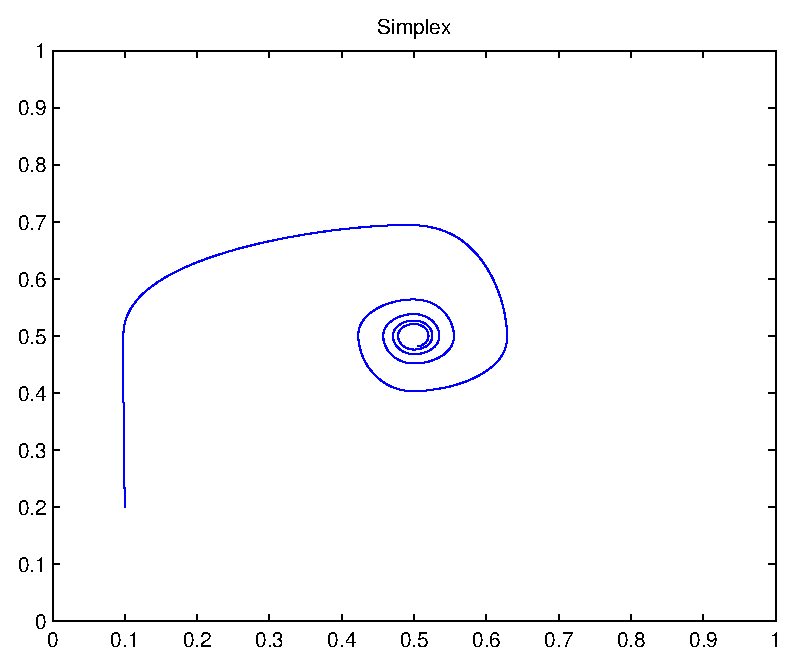
\includegraphics[width=\textwidth]{./images/test2_simplex_bnn.eps}
	  \caption{Simplex.}
	  \label{fig:test2_simplex_bnn}
  \end{subfigure}
  ~ 
  \begin{subfigure}[b]{0.45\textwidth}
	  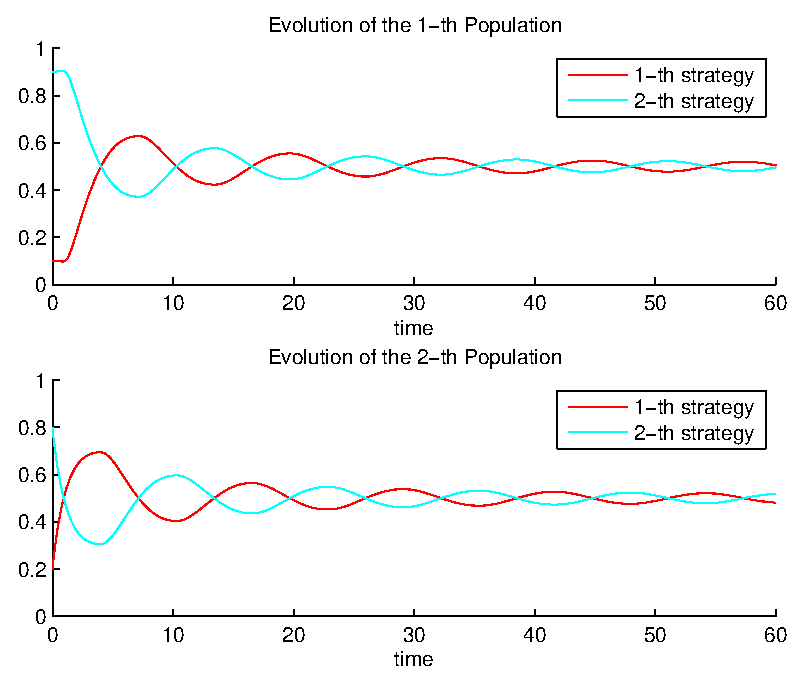
\includegraphics[width=\textwidth]{./images/test2_ev_bnn.eps}
	  \caption{Evolution of the strategies in time.}
	  \label{fig:test2_ev_bnn}
  \end{subfigure}
  \caption{Matching pennies game with BNN dynamics.}
  \label{fig:mp_game_bnn}
\end{figure}



\begin{figure}
  \centering
  \begin{subfigure}[b]{0.45\textwidth}
	  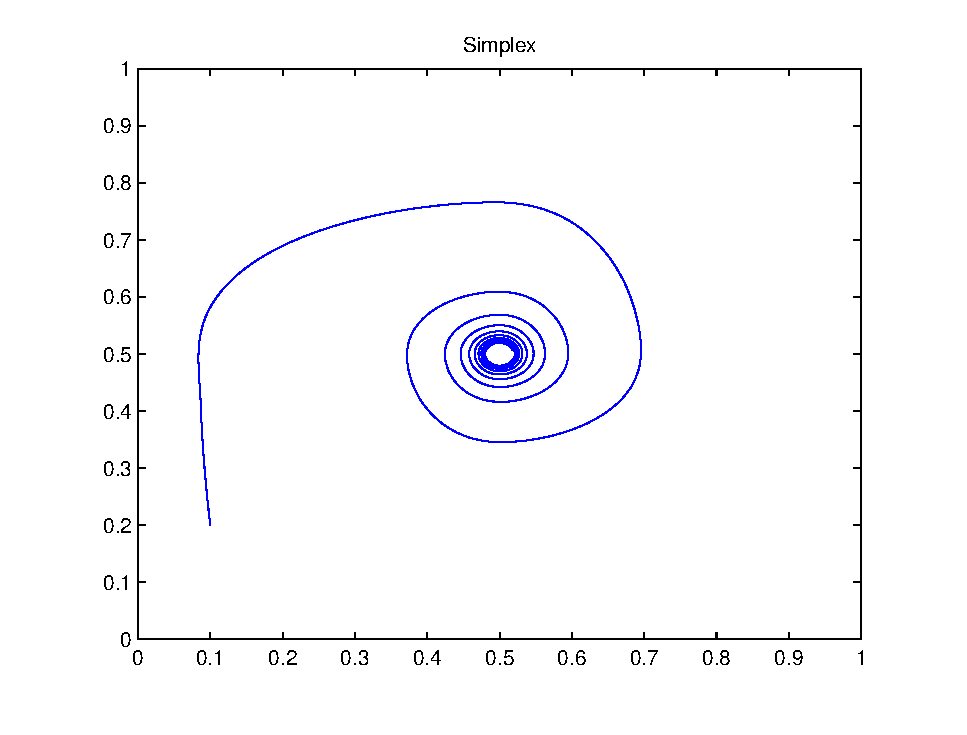
\includegraphics[width=\textwidth]{./images/test2_simplex_smith.eps}
	  \caption{Simplex.}
	  \label{fig:test2_simplex_smith}
  \end{subfigure}
  ~ 
  \begin{subfigure}[b]{0.45\textwidth}
	  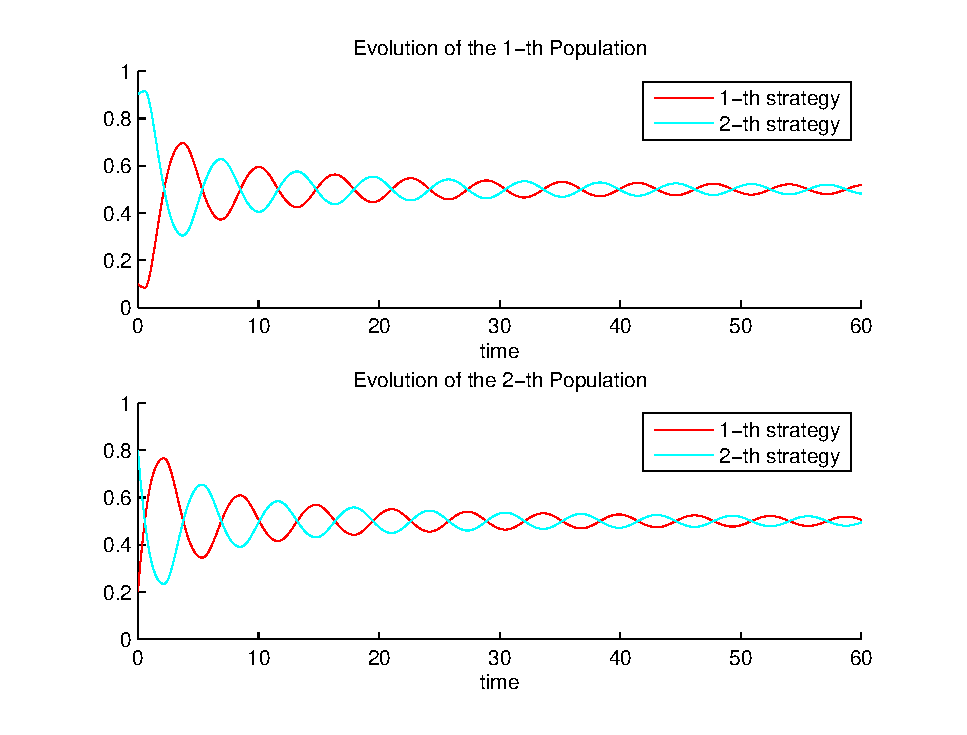
\includegraphics[width=\textwidth]{./images/test2_ev_smith.eps}
	  \caption{Evolution of the strategies in time.}
	  \label{fig:test2_ev_smith}
  \end{subfigure}
  \caption{Matching pennies game with Smith dynamics.}
  \label{fig:mp_game_smith}
\end{figure}



\begin{figure}
  \centering
  \begin{subfigure}[b]{0.45\textwidth}
	  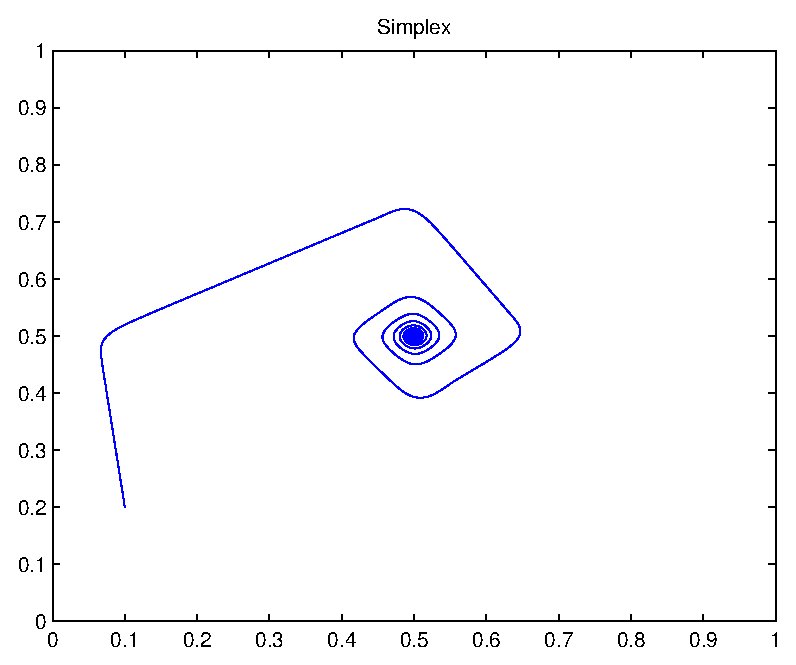
\includegraphics[width=\textwidth]{./images/test2_simplex_logit.eps}
	  \caption{Simplex.}
	  \label{fig:test2_simplex_logit}
  \end{subfigure}
  ~ 
  \begin{subfigure}[b]{0.45\textwidth}
	  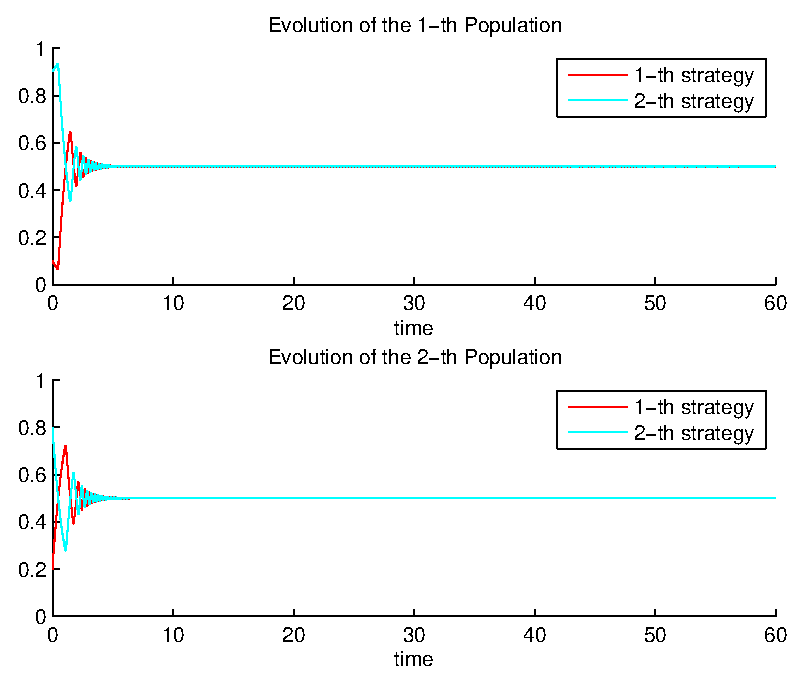
\includegraphics[width=\textwidth]{./images/test2_ev_logit.eps}
	  \caption{Evolution of the strategies in time.}
	  \label{fig:test2_ev_logit}
  \end{subfigure}
  \caption{Matching pennies game with logit dynamics.}
  \label{fig:mp_game_logit}
\end{figure}










\section{Designing games}

In the previous section we show some examples of strategical situations that can be analyzed with game theory. In these cases, the structure of the game is given by the problem. However, we can modify the fitness function of each player in order to solve an optimization problem.

For example, let us consider the following optimization problem:

\begin{equation}\label{eq:opt_problem}
\begin{aligned}
& \underset{x}{\text{maximize}} 
& & \sum_{i=1}^N U_i(x_i)  - C(|x|)\\
& \text{subject to}
& & 0 \leq q_i \geq m,  i =\{1,\ldots, N\}.
\end{aligned}
\end{equation}

This can be seen as a problem of allocating a finite resource to maximize a utility function. 

Note that there are $N$ agents with that give a valuation $v_i(x_i)$ to the resource $x_i$.

However, the cost of assigning the resource is $C(|x|)$ .

The cost of assigning the resource might be distributed among the population. 

Let us consider the following example:


\begin{equation}
U_i(x_i) =   \alpha_i  log(1+x_i) 
\end{equation}

\begin{equation}
C(z) = \beta z^2 + b z 
\end{equation}

define fitness functions as 

\begin{equation}
f_i(x_1, x_2) = \frac{\alpha_i}{1+x_i} - 2 \beta |x| - b 
\end{equation}


















\iffalse


      
\begin{figure}[htb]
 \includegraphics[1\textwidth]{./images/}
 \caption{}
 \label{fig:}
\end{figure}




test1_ev_bnn.eps         test1_simplex_rd.eps     test2_simplex_bnn.eps
test1_ev_logit.eps       test1_simplex_smith.eps  test2_simplex_logit.eps
test1_ev_rd.eps          test2_ev_bnn.eps         test2_simplex_rd.eps
test1_ev_smith.eps       test2_ev_logit.eps       test2_simplex_smith.eps
test1_simplex_bnn.eps    test2_ev_rd.eps
test1_simplex_logit.eps  test2_ev_smith.eps
\fi

\end{document}
